
\documentclass[12pt]{article}
\setlength\parindent{0pt}
\usepackage{fullpage}
\usepackage{amsmath}
\usepackage[margin=0.5in, paperwidth=13.5in, paperheight=8.4in]{geometry}
\usepackage{graphicx}
\setlength{\parskip}{4mm}
\def\LL{\left\langle}   % left angle bracket
\def\RR{\right\rangle}  % right angle bracket
\def\LP{\left(}         % left parenthesis
\def\RP{\right)}        % right parenthesis
\def\LB{\left\{}        % left curly bracket
\def\RB{\right\}}       % right curly bracket
\def\PAR#1#2{ {{\partial #1}\over{\partial #2}} }
\def\PARTWO#1#2{ {{\partial^2 #1}\over{\partial #2}^2} }
\def\PARTWOMIX#1#2#3{ {{\partial^2 #1}\over{\partial #2 \partial #3}} }
\newcommand{\BE}{\begin{displaymath}}
\newcommand{\EE}{\end{displaymath}}
\newcommand{\BNE}{\begin{equation}}
\newcommand{\ENE}{\end{equation}}
\newcommand{\BEA}{\begin{eqnarray}}
\newcommand{\EEA}{\nonumber\end{eqnarray}}
\newcommand{\EL}{\nonumber\\}
\newcommand{\la}[1]{\label{#1}}
\newcommand{\ie}{{\em i.e.\ }}
\newcommand{\eg}{{\em e.\,g.\ }}
\newcommand{\cf}{cf.\ }
\newcommand{\etc}{etc.\ }
\newcommand{\Tr}{{\rm tr}}
\newcommand{\etal}{{\it et al.}}
\newcommand{\OL}[1]{\overline{#1}\ } % overline
\newcommand{\OLL}[1]{\overline{\overline{#1}}\ } % double overline
\newcommand{\OON}{\frac{1}{N}} % "one over N"
\newcommand{\OOX}[1]{\frac{1}{#1}} % "one over X"

\pagenumbering{gobble}

\begin{document}
\Large
\centerline{\sc{Recitation Exercises}}
\normalsize
\centerline{\sc{Wednesday, 12 May}}

Consider a vibrating string that is 72 cm long; it is stretched so that the frequency of its fundamental mode ($n=1$) is 293 Hz. Below, I have drawn the fundamental mode of that string for you. Determine its wavelength. Then, draw the next three resonant modes, and determine their frequencies and wavelengths.
\vspace{0.5in}


\begin{minipage}{0.5\textwidth}
	\begin{center}
\Large		Vibration pattern
	\end{center}
\end{minipage}
\begin{minipage}{0.25\textwidth}
	\Large \begin{center}Wavelength\end{center}
\end{minipage}
\begin{minipage}{0.25\textwidth}
\Large	\begin{center}Frequency\end{center}
\end{minipage}


\begin{minipage}{0.5\textwidth}
	\begin{center}
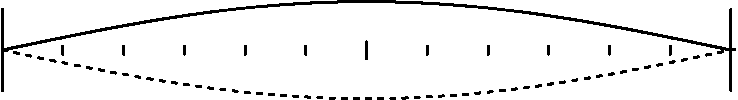
\includegraphics[width=0.9\textwidth]{fund-crop.pdf}
	\end{center}
\end{minipage}
\begin{minipage}{0.25\textwidth}
\hspace{0.5in}
\end{minipage}
\begin{minipage}{0.25\textwidth}
\begin{center}
	\Large 293 Hz
\end{center}	
\end{minipage}

\vspace{0.5in}
\begin{minipage}{0.5\textwidth}
	\begin{center}
		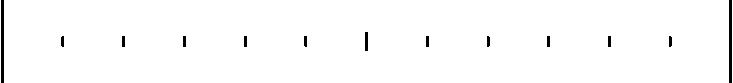
\includegraphics[width=0.9\textwidth]{string-crop.pdf}
	\end{center}
\end{minipage}
\begin{minipage}{0.25\textwidth}
	\hspace{0.5in}
\end{minipage}
\begin{minipage}{0.25\textwidth}
	\begin{center}

	\end{center}	
\end{minipage}


\vspace{0.5in}
\begin{minipage}{0.5\textwidth}
	\begin{center}
		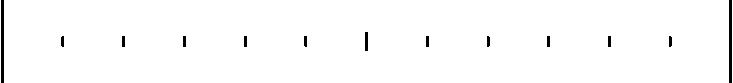
\includegraphics[width=0.9\textwidth]{string-crop.pdf}
	\end{center}
\end{minipage}
\begin{minipage}{0.25\textwidth}
	\hspace{0.5in}
\end{minipage}
\begin{minipage}{0.25\textwidth}
	\begin{center}
		
	\end{center}	
\end{minipage}


\vspace{0.5in}
\begin{minipage}{0.5\textwidth}
	\begin{center}
		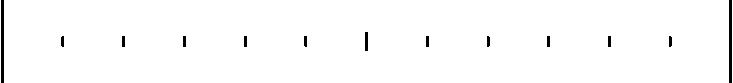
\includegraphics[width=0.9\textwidth]{string-crop.pdf}
	\end{center}
\end{minipage}
\begin{minipage}{0.25\textwidth}
	\hspace{0.5in}
\end{minipage}
\begin{minipage}{0.25\textwidth}
	\begin{center}
		
	\end{center}	
\end{minipage}

\newpage

The human hearing range extends from 20 Hz to around 20 kHz, with the upper limit declining gradually with age and exposure to loud sounds. In music, the important thing for our perception of melody and harmony is the {\it fundamental frequency} of the notes being played. The fundamental frequencies of strings on a piano range from 27.5 Hz to 8372 Hz. However, music rarely uses the notes at the edge of the piano; the fundamental frequencies of the notes most common in music range from perhaps 70 Hz (about two octaves below middle C, an extremely low note for a bass voice) to 1000 Hz (about two octaves above, a high note for a soprano voice).

However, small speakers have difficulty producing low frequencies. Suppose that a certain cellphone's small speaker can't produce sounds below 250 Hz.

Suppose a trombone player plays a note with a fundamental frequency of 100 Hz (around G below C below middle C). Trombones produce a lot of energy in many different normal modes. Imagine that you record that note on the trombone and play it back on this cellphone that cannot produce frequencies below 250 Hz. 

Would someone be able to hear it? If not, describe why. If they would be able to hear it, describe some of the frequencies they would hear.

\vspace{1.5in}

Would this listener be able to determine that the fundamental frequency of the note was 100 Hz rather than some other value? How?

\vspace{1.5in}

\newpage

A person with this sort of cellphone -- again, unable to reproduce low frequencies -- listens to their phone and hears what sounds like two notes being played at once. The lowest frequencies they hear are {\bf 320, 360, 480, 600, 640, 720, 800, 840, 960, 1080, 1120, and 1200 Hz}. (Keep in mind there were some other frequencies present in the original signal that the cellphone was unable to reproduce.)

What are the fundamental frequencies of the two notes that were played? To help you, label the frequencies you hear with horizontal lines on the scale to the right, as you have seen from the spectrogram in class.

In trying to figure out the two fundamental frequencies present, it may help to mark which frequency you think goes with which note on the scale below.

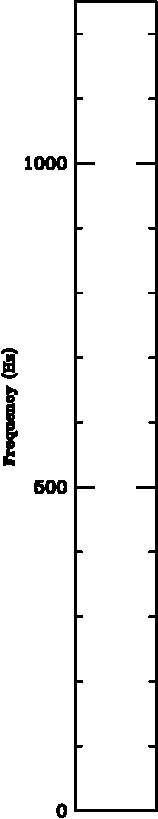
\includegraphics[width=1.1in]{scale.pdf}


 \end{document}
